\documentclass[twocolumn]{article}
\usepackage{graphics}
\usepackage{graphicx}
\usepackage[utf8]{inputenc}
\usepackage{hyperref}
\usepackage{natbib}
\usepackage{graphicx}
\usepackage{svg}
%%\usepackage{floatrow}

\graphicspath{ {./assets/images/} }

%links
\hypersetup{
    colorlinks=true,
    linkcolor=blue,
    filecolor=magenta,      
    urlcolor=cyan,
}

%Pseudocode
\usepackage[german,vlined,longend,ruled,linesnumbered]{algorithm2e}
\SetKw{KwDownTo}{downto}
\SetKw{KwAnd}{and}
\SetKw{KwOr}{or}
\SetKwBlock{DoParallel}{do in parallel}{end}
\usepackage{xcolor}
\newcommand\mycommfont[1]{\footnotesize\ttfamily\textcolor{blue}{#1}}
\SetCommentSty{mycommfont}
\DontPrintSemicolon

\newcommand{\aetitle}{Efficient updating Customizable Contraction Hierarchies} % Title of the 

\newcommand{\studentOne}{Marius Hahn} % Name 2
%\newcommand{\studentTwo}{Efficient updating Customizable Contraction Hierarchies} % Name 2


% Bis zum 19.07. soll ein kurzer Report abgegeben werden (ca. 2 Seiten), der das zugewiesene
% Thema kritisch betrachtet und Limitation der vorgestellten Algorithmem analysiert, z.B. hinsichtlich 
% der Performanz. Außerdem sollen mögliche auf dem Paper basierende weitergehende Forschungsfragen
% benannt werden.

\begin{document}

\twocolumn[{\begin{small}
                \begin{minipage}{0.5 \linewidth}
                    Seminar Summer Term 2022
                \end{minipage}
                \begin{minipage}{0.5\linewidth}
                    \begin{flushright}
                        \studentOne
                    \end{flushright}
                \end{minipage}
            \end{small}}
        {\begin{center}
                \begin{sffamily}\Large\bfseries \aetitle \end{sffamily}
            \end{center}}
    \vskip 3em]

\section{Intro}

This is a seminar on "Efficient shortest path index maintenance on dynamic
road networks with theoretical guarantees" \cite{Ouyang2020}. The papers generally is
about finding the shortest path in road networks. By \textit{shortest} it is meant,
the path that requires the less time to get from source $s$ to a target $t$. The route
network is modeled as a directed graph $G(V,E)$ where each street crossing represents a
vertex $v \epsilon V$ and each road between crossings represents an edge $e \epsilon E$.
The most basic and solid method to find shortest paths between vertices in a graph is
Dijkstra's algorithm \cite{Dijkstra1959}. This algorithm is proofed to always return the
correct shortest path but it is not fast enough for just in time route planning on large
road networks as we know it from services like Google Maps.
\\
There are many
different approaches that try to speed up shortest path queries by precomputing
any different kind of index structure before doing the shortest path query. The index
structure discussed in here \cite{Ouyang2020} is CH (Contraction Hierarchies)\cite{Geisberger}
with some extension. This extension is CCH (Customizable Contraction Hierarchies)
\cite{Dibbelt2014}. Although the authors of \cite{Ouyang2020} never mention the term
CCH their approaches builds the same index structure. This is a pity, as for this part
they kind of reinvent the wheel.
\\
The difference lies in updating
the CCH index structure. For updating the CCH, the authors of \cite{Ouyang2020} will use yet another
index structure called \textit{SS-Graph} that helps to exactly identify the shortcuts that
have to be updated, after some edge weight has changed. In todays implementation, the whole
index structure is recomputed periodically. This is an valid approach as it is fast enough
to stay accurate for route planning in road networks.
\\
In \cite{Ouyang2020} the authors would like to find a way that make it possible to handle streaming
updates. Therefore it is necessary to handle streaming updates, meaning handle single weight decrease
and increases. To do so another index structure the \textit{SS-Graph} is introduced.
This index structure is a helper structure to identify the shortcuts
that have to be updated in the CCH.
\\
The disadvantage of this \textit{SS-Graph} is that the overall space consumption rises.
This can be a deal breaker for large networks.
Finally they introduce a way to create the necessary \textit{SS-Graph} on the fly. Which
is only a part of the whole structure.
Sadly the exact way, how, is missing in the paper \cite{Ouyang2020}.


\section{Shortcut Supporting Graph}

\begin{figure}[h]
    \caption{Base Graph $G$}
    \centering
    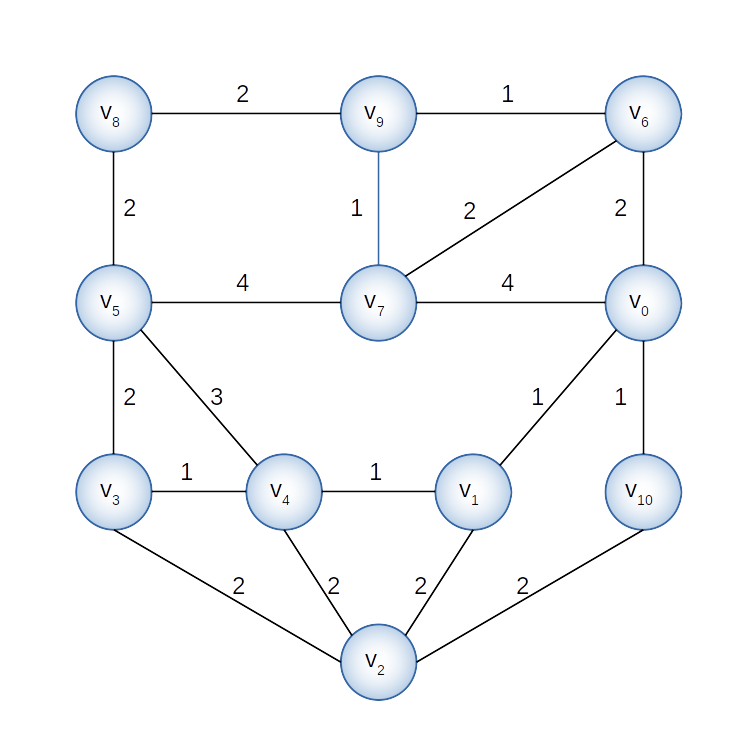
\includegraphics[width=\linewidth]{baseGraph}
    \label{fig:baseGraph}
\end{figure}

This section is about the \textit{Shortcut Supporting Graph} introduced in \cite{Ouyang2020}.
The way how the shortcut index is created is omitted because it is a Customizable Contraction
Hierarchies shortcut index and therefore not of further interest. Although the algorithm to get
there is described differently the result is a shortcut index that encodes every simple path.
This is the same in CCH.
\\
Figure \ref{fig:baseGraph} represents the sample base graph on which is used as an example graph 
throughout this whole work. It is the same as used in \cite{Ouyang2020}, but redrawn.


\begin{figure}[h]
    \caption{Shortcut Index Graph $G'$}
    \centering
    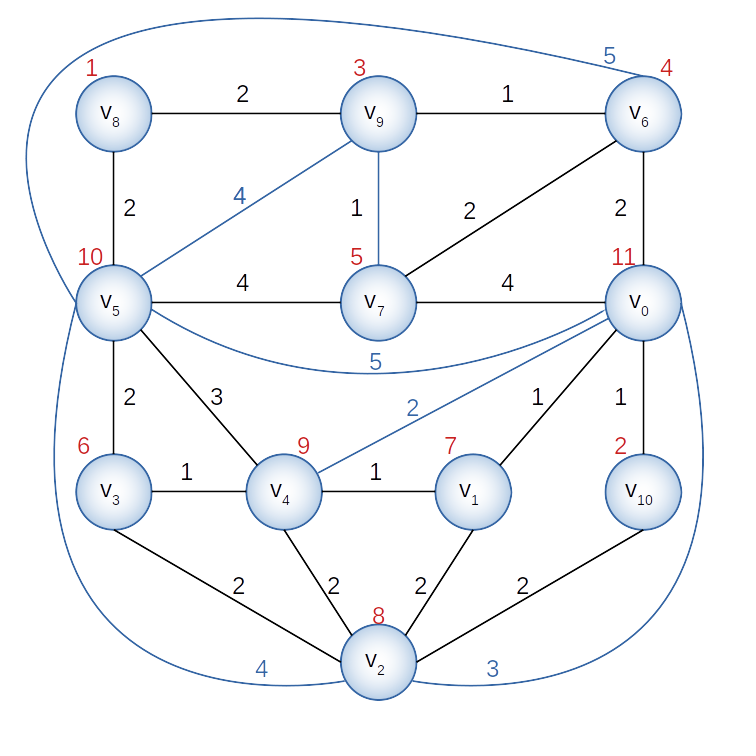
\includegraphics[width=\linewidth]{cchGraph}
    \label{fig:shortcutIndex}
\end{figure}

Figure \ref{fig:shortcutIndex} represents the \textit{Shortcut Index G'} already materialized. The red numbers
located just outside the vertices represent the contraction order. The numbers on the edge are the weight
assigned to the edge. The inserted shortcuts are drawn in blue and have their weight already assigned, too.

Based on this \textit{Shortcut Index G'} yet another index structure is introduced. The \textit{Shortcut Supporting Graph G*}.
$G*$ is a directed graph that has two different kind of vertices. The first vertex set $V_s$ represents all the
edges that are contained in the \textit{Shortcut Index G'}. The second vertex set are the relation type 
vertices $V_r$. A relation type vertex $v_r$ has two in-neighbors $v_{s1}$ and $v_{s2}$ that and one 
out neighbor $v_{s3}$. Each vertex in $V_s$ has three properties. 

\begin{itemize}
    \item The edge or shortcut $e = (v_u, v_v)$ in $G'$ it represents
    \item The shortest path cost $\phi(e)$ 
    \item The numbers of relation type vertices that support this edge or shortcut and lye on the shortest path $c_{\phi}(e)$
\end{itemize}

Figure \ref{fig:SsGraph} is the \textit{Shortcut Supporting Graph G*} of \textit{Shortcut Index G'}.
\\
\textbf{Example 1:} Lets take this most upper vertex of $G*$ in figure \ref{fig:SsGraph}. It represents
the shortcut $e= (v_0, v_5)$. This shortcut is supported through four other simple paths in G' of two hops.
\begin{enumerate}
    \item $R_1$ with the two in neighbors $v_{s1} = (v_7, v_5)$ and $v_{s2} = (v_7, v_0)$ with total path cost $\phi = \phi(v_{s1}) + \phi_{v_{s2}} = 8$
    \item $R_2$ with the two in neighbors $v_{s1} = (v_4, v_5)$ and $v_{s2} = (v_4, v_0)$ with total path cost $\phi = \phi(v_{s1}) + \phi_{v_{s2}} = 5$
    \item $R_5$ with the two in neighbors $v_{s1} = (v_6, v_5)$ and $v_{s2} = (v_6, v_0)$ with total path cost $\phi = \phi(v_{s1}) + \phi_{v_{s2}} = 7$
    \item $R_6$ with the two in neighbors $v_{s1} = (v_2, v_5)$ and $v_{s2} = (v_0, v_5)$ with total path cost $\phi = \phi(v_{s1}) + \phi_{v_{s2}} = 7$
\end{enumerate}

$c_{\phi}(e) = 1$ as only $R_2$ is on the shortest path that has length five. 

\begin{figure*}[t]
    \caption{Shortcut Support Index $G*$}
    \centering
    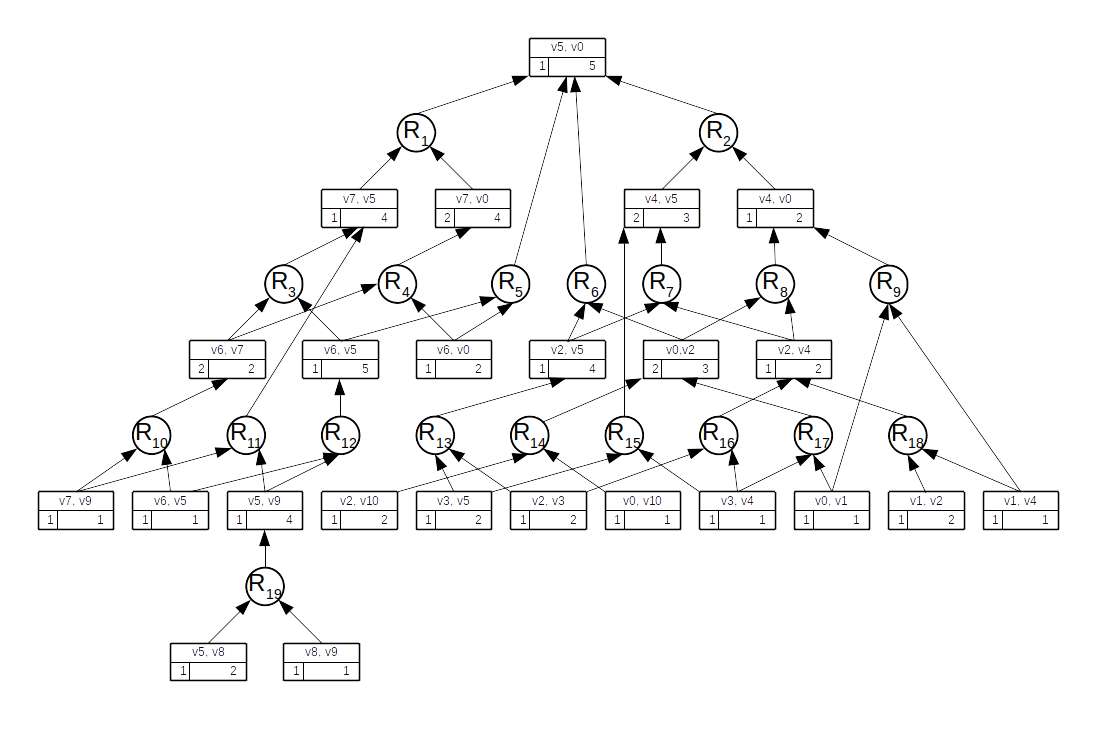
\includegraphics[width=\textwidth]{SsGraph}
    \label{fig:SsGraph}
\end{figure*}

\subsection{Space Complexity}

The space consumption of $G*$ is: 
\\
$\mathcal{O}(\vert E(G') \vert + \sum_{v \epsilon  V(G')}(\vert Nbr(v) \vert * (\vert Nbr(v) \vert-1)/2))$
where $Nbr(v) = {u\vert u \epsilon nbr(v) \land \gamma(u) > \gamma(v) }$ and $\gamma(u)$ is the rank of vertex $u$.
This is a lot more than $G'$ and can be a problem in practice. There exists a method to get this build the needed
part of this graph on the fly while updating the edges. 

\section{Reaction on Weight Changes}

Here we will have a look what happens on a weight decrease or increase. 
In CCH for the whole shortcut index is updated in a fixed time interval. We want to 
do streaming updates which means reaction to a single weight change. In classic
CCH you usually have to recontract at least all vertices with a higher rank than
the once that form the endpoint of the updated edge. Having the \textit{Shortcut Support Index $G*$}
it is possible to determine which edges have to be updated. In general this could
be the same amount of edges but in real applications this is very unlikely.

\subsection{Weight Decrease}

In this case a single edge weight decrease. The algorithm in figure \ref{fig:decreaseAlgorithm} 
show what to do in this case. The update of the support counter $c_{\phi}$ is omitted as
figure \ref{fig:decreaseAlgorithm} is copied from \cite{Ouyang2020} and it was omitted there, too. The support counter $c_{\phi}$
isn't needed for the decrease case to work but it is needed in the decrease case to later on 
work together with the increase case. Fixing this is out of the scope for this work. Therefore the 
algorithm is presented as is in figure \ref{fig:decreaseAlgorithm}. 

\begin{figure}[ht]
    \caption{Shortcut Index Graph $G'$}
    \centering
    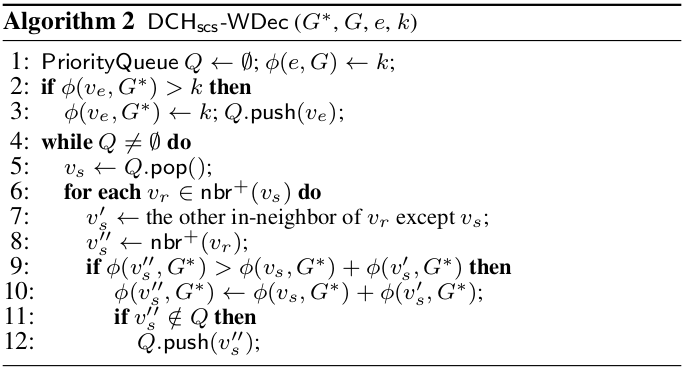
\includegraphics[width=\linewidth]{decreaseAlgorithm}
    \label{fig:decreaseAlgorithm}
\end{figure}

What this algorithm basically dose is, when a weight decreases it looks for shortcuts that are build upon this edge.
If the weight of this shortcut doesn't depend on the edge it stops. If the weight of this shortcut depends on the edge, 
meaning the edge was lying on the shortest path, it updates the weight of the shortcut. This happens recursively.

This guarantees that only edges that are one hop dependent on a changed edge are explored. Therefore the time complexity 
of this algorithm is $\mathcal{O}(\vert\Delta\vert  * (log \vert \Delta \vert + deg'_{max}) + 1)$.  $\vert\Delta\vert$ is the
number of shortcuts that have to be updated and $deg'_{max}$. 
% In the worst case $\vert\Delta\vert$ are all edges and shortcuts have a vertex involved with a higher rank than in the changed edge $e$.

\subsection{Weight increase}
In this case a single edge weight increase. The algorithm in figure \ref{fig:increaseAlgorithm} 
show what to do in this case. 

\begin{figure}[ht]
    \caption{Shortcut Index Graph $G'$}
    \centering
    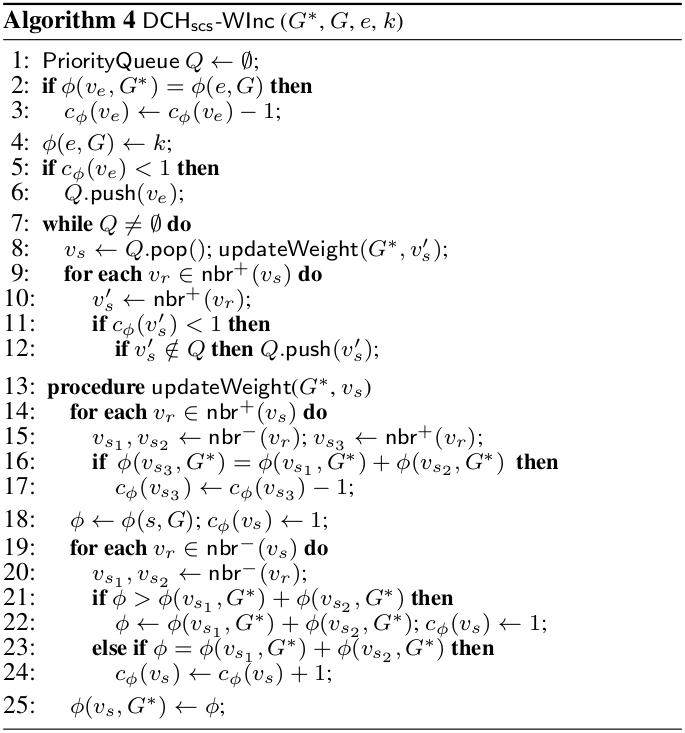
\includegraphics[width=\linewidth]{increaseAlgorithm}
    \label{fig:increaseAlgorithm}
\end{figure}


\section{Experimental Results}

The experimental re

\newpage

\bibliographystyle{plain}
\bibliography{assets/references}
\listoffigures

\end{document}
